\begin{frame}
\frametitle{Internet Control Message Protocol}
ICMP è un protocollo che opera al livello di rete (livello 3 modello ISO/OSI), 
e permette la segnalazione di  errori, la diagnostica della rete e la 
messaggistica di controllo. Date queste caratteristiche risulta fondamentale 
per il funzionamento, il monitoraggio e la diagnostica delle reti IP e che, 
proprio per questo, non può essere completamente disabilitato o filtrato 
nelle reti moderne senza comprometterne l'operatività. 
Tutto ciò lo rende un candidato ideale per la creazione di canali di 
comunicazione nascosti e difficilmente rilevabili. 
%L'implementazione di un Covert Channel è possibile siccome è un protocollo 
%che molti firewall e dispositivi di sicurezza consentono. Dati i suoi 
%utilizzi, non può essere del tutto disabilitato. 
\vspace{1ex} \newline 
Successivamente verrà mostrato come il protocollo è stato sfruttato per 
l'implementazione di diverse tipologie di Covert Channel.
\end{frame} 
\begin{frame}
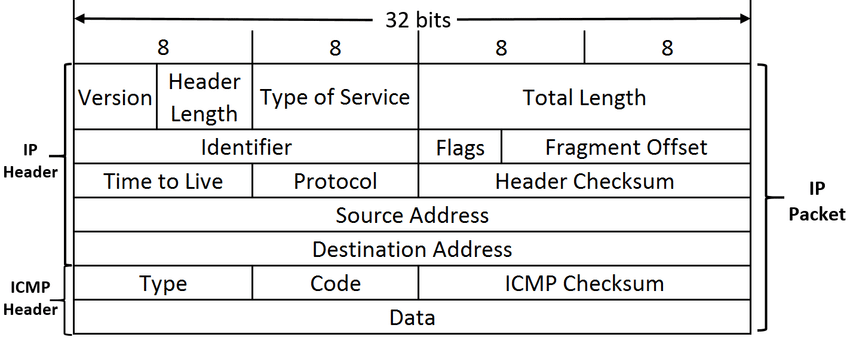
\includegraphics[width=0.9\textwidth]{../Tesi/img/ICMP-packet-structure.png} 
\captionof{figure}{Struttura di un messagio ICMP}
\end{frame} 
\begin{frame} 
\begin{longtable}{|p{0.2\textwidth}|p{0.7\textwidth}|} 
    \hline
    \textbf{Utilizzi} & \textbf{Descrizione} \\
    \hline
    Diagnostica della rete & Fornisce metriche critiche per il monitoraggio continuo delle prestazioni della rete  
    \\ \hline 
    Segnalazione di errori &  Rileva e segnala i problemi riscontrati durante la trasmissione dei dati tra i dispositivi sulla rete 
    \\ \hline
    Risoluzione dei problemi & Gli amministratori di rete possono ricevere avvisi in tempo reale e rispondere rapidamente ai problemi di rete grazie agli strumenti di monitoraggio basati su ICMP. 
    \\ \hline
    Ottenimento di informazioni & Invia messaggi e informazioni senza la necessità di una connessione preventiva. 
    \\ \hline 
\caption{Utilizzi del protocollo ICMP}  
\end{longtable} 
\end{frame} 